%
%	Documento de análisis (diagramas)
%

\documentclass[11pt, a4paper, twoside, titlepage]{article}
\usepackage[utf8x]{inputenc}
\usepackage[T1]{fontenc}
\usepackage[spanish, es-ucroman]{babel}
\usepackage{lmodern}
\usepackage{anysize}
\usepackage{fancyhdr}
\usepackage[none]{hyphenat}
\usepackage[colorlinks, linkcolor=red]{hyperref}
\usepackage{float}
\usepackage{lscape}
\usepackage{pdflscape}
\usepackage[doc=analisis]{isdiedral}

% Nombre del documento (para futuras referencias)
\newcommand*{\doctitle}{Análisis}
\newcommand*{\docversion}{1.1}


%%% Configuraciones %%%
\marginsize{2.5cm}{2cm}{2cm}{2cm}

% Usa como familia tipográfica por defecto "Sans"
\renewcommand{\familydefault}{\sfdefault}

% Establece la profundidad hasta la cual se numeran los elementos de sección
\setcounter{secnumdepth}{4}

% Establece la profundidad de niveles de sección que aparece en el TOC
\setcounter{tocdepth}{4}

% Configuración de los encabezados
\encabezadodiedral{\doctitle{} \docversion}
\pagestyle{fancy}

\renewcommand*{\thepage}{\sffamily \roman{page}}

\title{\doctitle\\\textsl{Airline Common Environment}}
\author{Grupo Diedral}

% Metadatos del pdf
\hypersetup{
pdfinfo={
	Author={Grupo Diedral},
	Title={\doctitle{} \docversion},
	Subject={Airline Common Environment},
	Keywords={análisis, UML, Airline Common Environment, Ingeniería del Software}
}
}

\begin{document}
	% Tabla de cambios
	\begin{tablacambios}
		1.0 & 28 de abril de 2013 & Todos & Versión inicial \\ \hline
		1.1 & 13 de mayo de 2013  & Todos & Correcciones puntuales
	\end{tablacambios}

	% Cita inicial
	\fijacitainicial{Para mostrar este diagrama adecuadamente, necesitaría una pantalla de cuatro dimensiones. Sin embargo, debido a los recortes del gobierno, nos tendremos que conformar con una pantalla bidimensional}{\emph{Historia del tiempo}, Stephen Hawking}

	% Portada
	\portadaace{\doctitle}{\docversion}

	\tableofcontents
	\newpage

	\iniciarnumeraciondiedral

	\begin{prologo}
		Este documento recoge la documentación generada durante la fase de análisis del proyecto. En primer lugar se incluye el diagrama de modelo de dominio que presenta y relaciona los conceptos generales relacionados con el dominio del producto. A continuación se introduce el diagrama de paquetes. Finalmente se muestra el análisis detallado del paquete {\itshape Gestión Externa}, incluyendo el diagrama de clases y los diferentes diagramas de comunicación correspondientes a cada caso de uso.\\

		Esta información ha sido especificada por medio del \itshape{Lenguaje Unificado de Modelado} (UML).

	\paragraph*{Nota sobre herramientas empleadas:} para la elaboración de los diagramas se ha utilizado el\break programa {\normalfont BoUML} en su versión {\normalfont 4.23 patch 7 `ultimate'}.
	\end{prologo}

	\section{Diagrama de modelo de dominio}
		\begin{figure}[H]\centering
			\hspace*{-.5cm}
			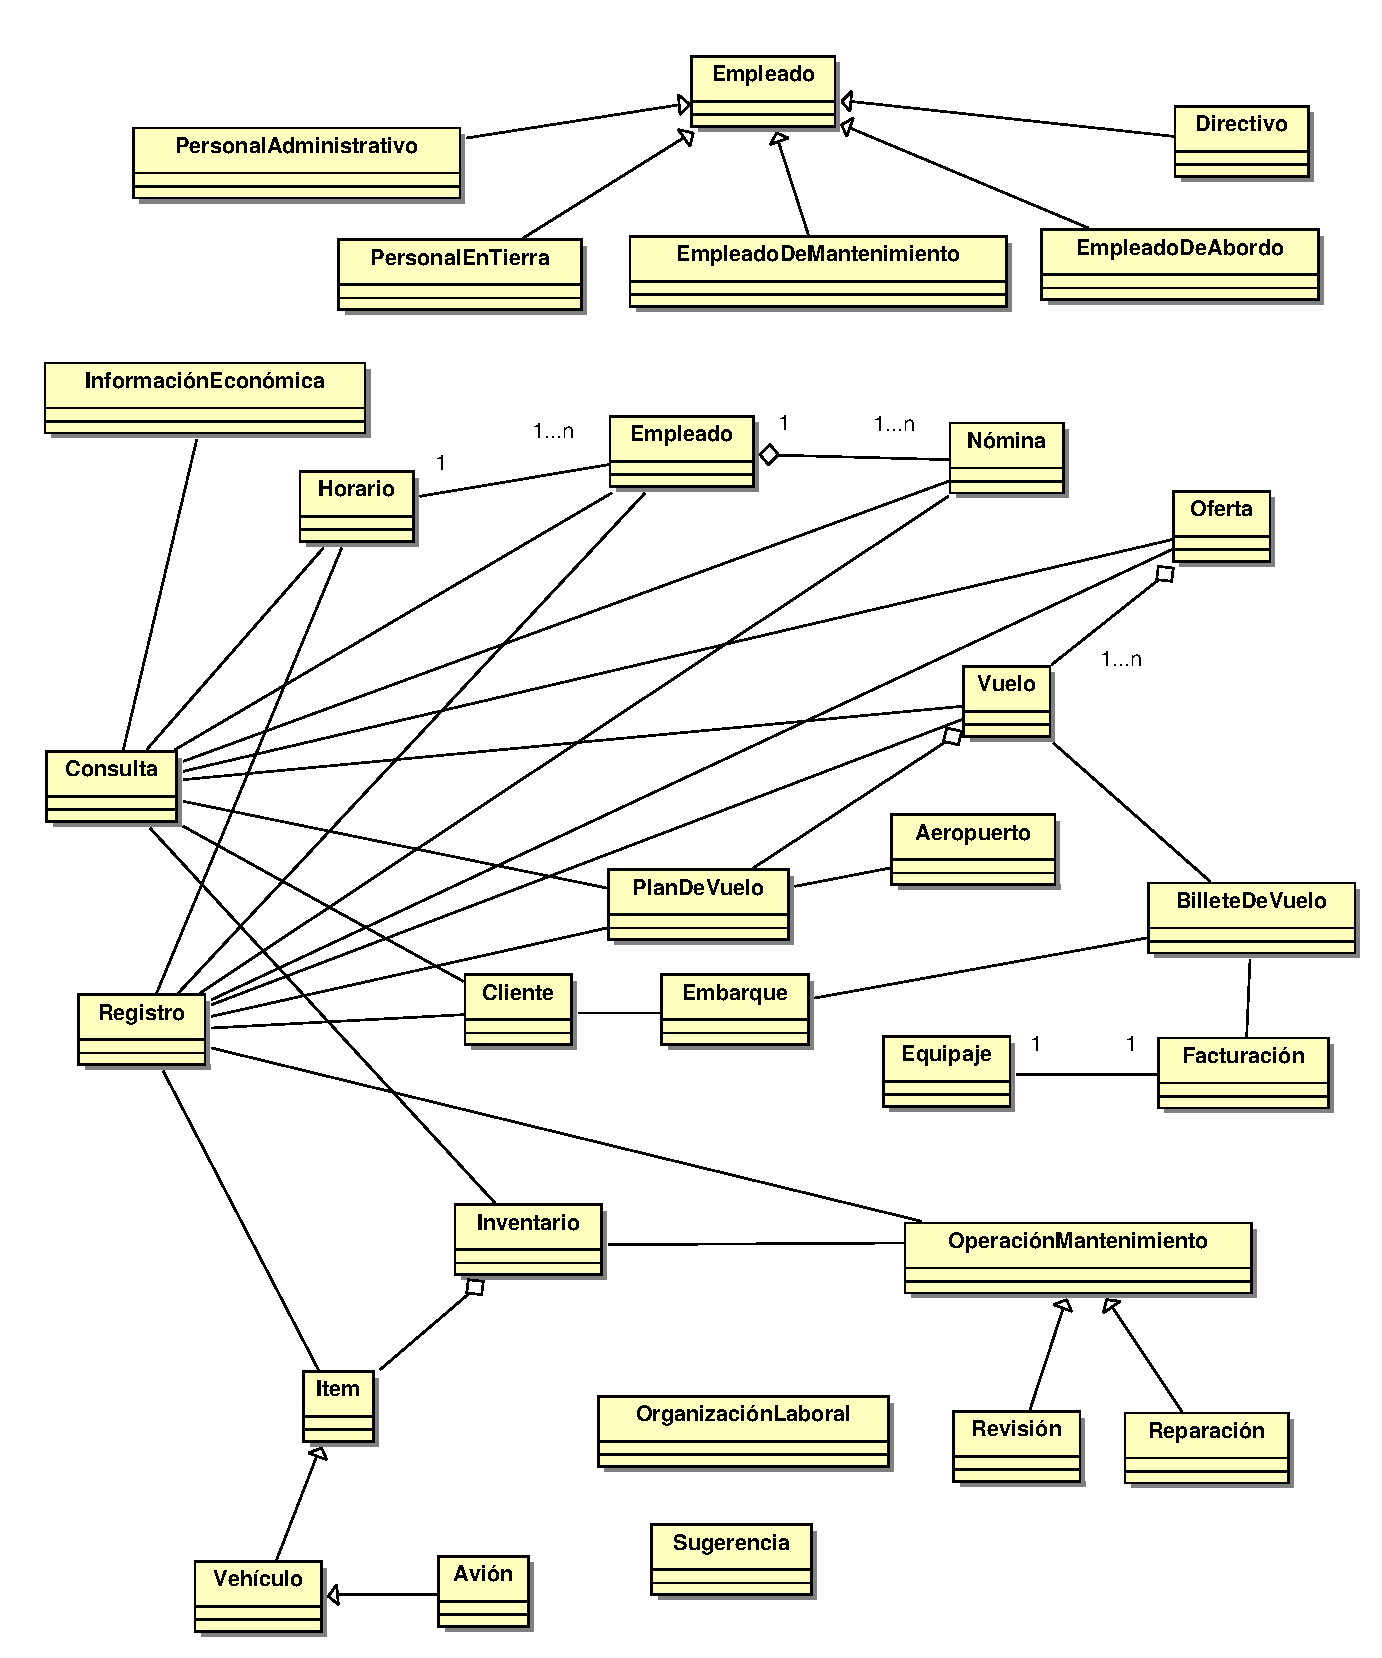
\includegraphics[scale=.722]{diagramas/modelodominio.pdf}
		\end{figure}	
	\newpage

\begin{landscape}
	\section{Diagrama de paquetes}
		\vfill
		\begin{figure}[H]\centering
			\hspace*{-.5cm}
			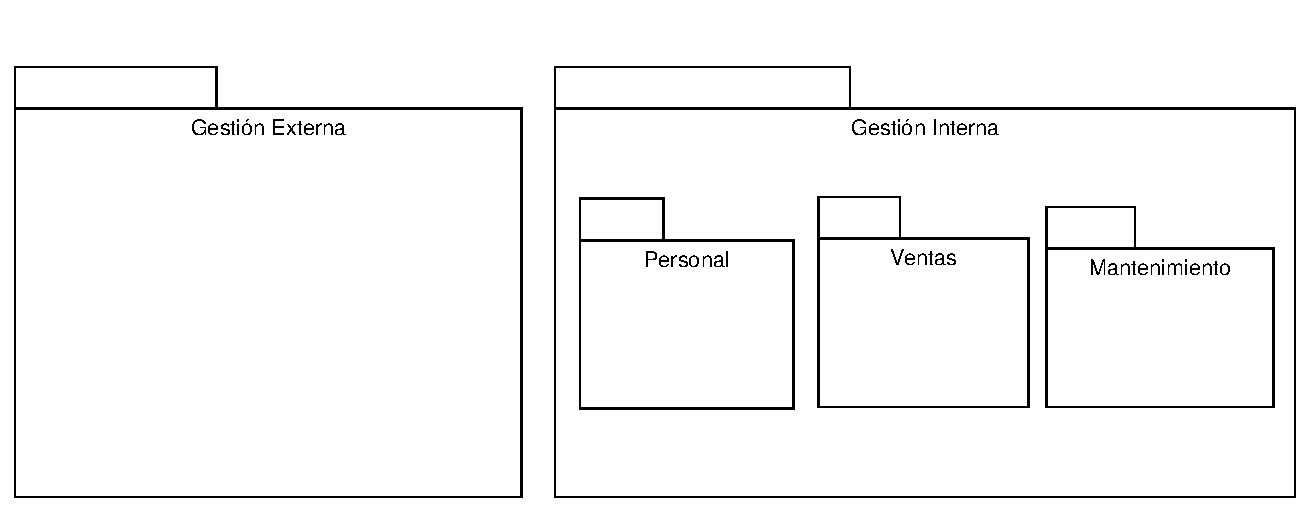
\includegraphics[scale=1]{diagramas/paquetes.pdf}
		\end{figure}
		\vfill
\end{landscape}
	\newpage

\begin{landscape}
	\section{El paquete {\itshape Gestión Interna}}
		\subsection{Diagrama de clases}

			\begin{figure}[H]\centering
				\vspace{2cm}
				\hspace{-2cm}
				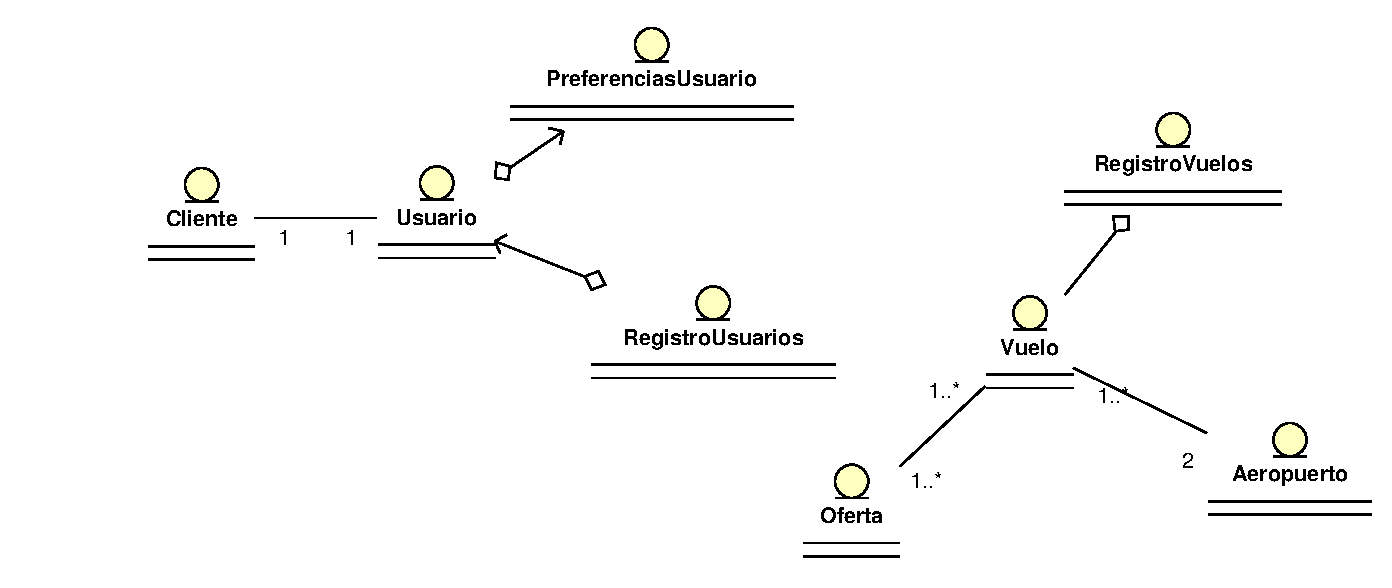
\includegraphics[scale=1]{diagramas/diagramaclases.pdf}
			\end{figure}		
\end{landscape}
\begin{landscape}
			\begin{figure}[H]\centering
				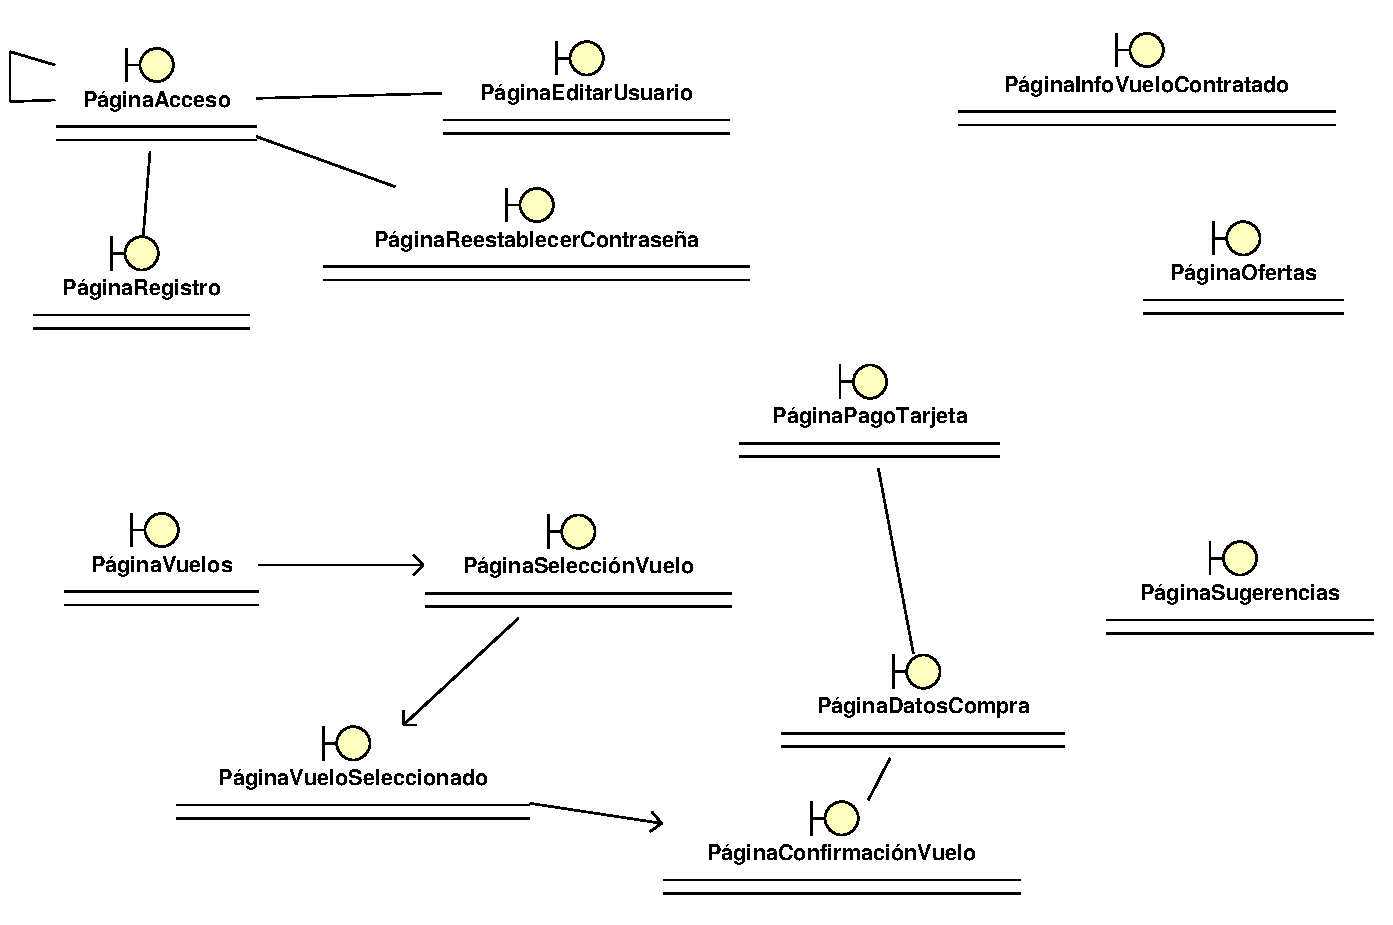
\includegraphics[scale=1]{diagramas/sitioweb.pdf}
			\end{figure}
\end{landscape}

		\subsection{Diagramas de comunicación}

			\subsubsection{Acceder web}
				\begin{figure}[H]\centering
					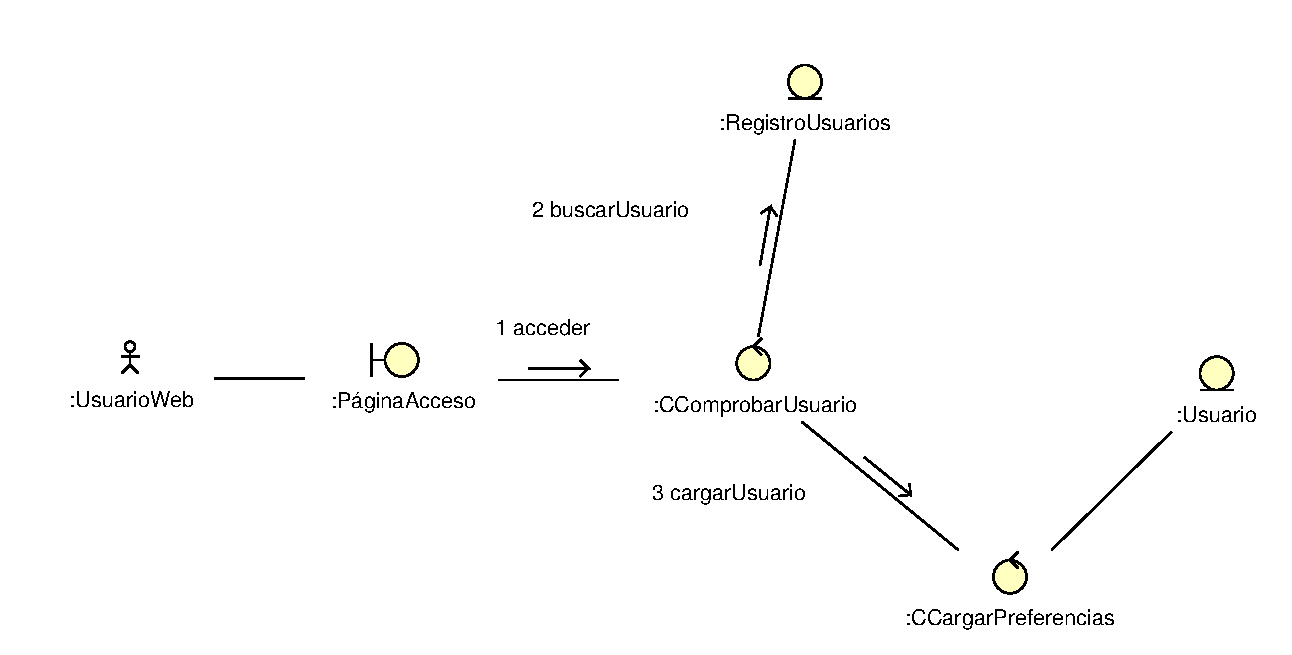
\includegraphics[scale=.75]{diagramas/accederweb.pdf}
				\end{figure}

				A través de la interfaz {\itshape PáginaAcceso} el usuario introduce sus datos de identificación personal (a saber, su nombre de usuario y contraseña). El sistema busca en la base de datos de usuarios registrados (representada en {\itshape RegistroUsuarios}) un usuario que se corresponda con los datos aportados. Si fuese necesario se cargarían las preferencias personales del usuario. Al finalizar la secuencia el usuario tiene una sesión activa que le da acceso a otras características de la aplicación.

				La entidad {\itshape Usuario} representa a un usuario registrado de la página web, que no es necesariamente un cliente. La entidad lo representa por medio de unos datos personales básicos como puede ser un identificador único, una clave secreta y una dirección de contacto.

			\subsubsection{Comprar billete}
				\begin{figure}[H]\centering
					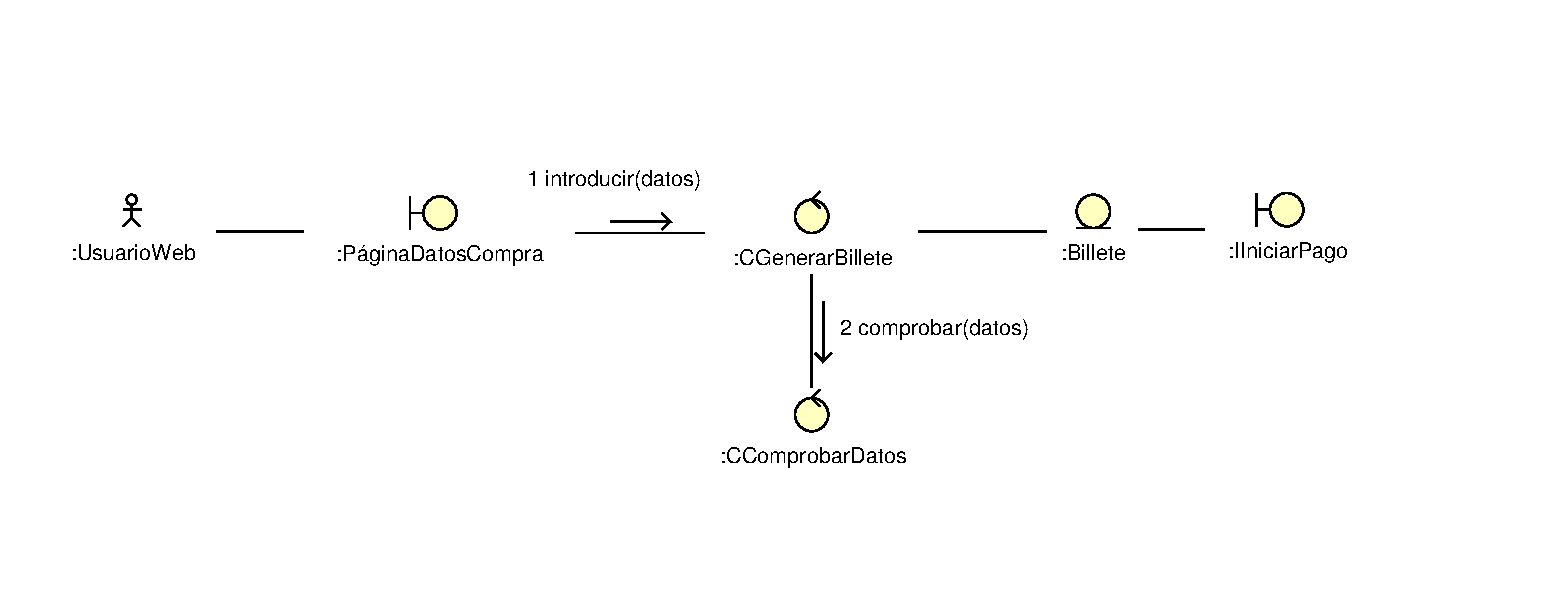
\includegraphics[scale=.72]{diagramas/comprarbillete.pdf}
				\end{figure}

			\subsubsection{Consultar oferta}
				\begin{figure}[H]\centering
					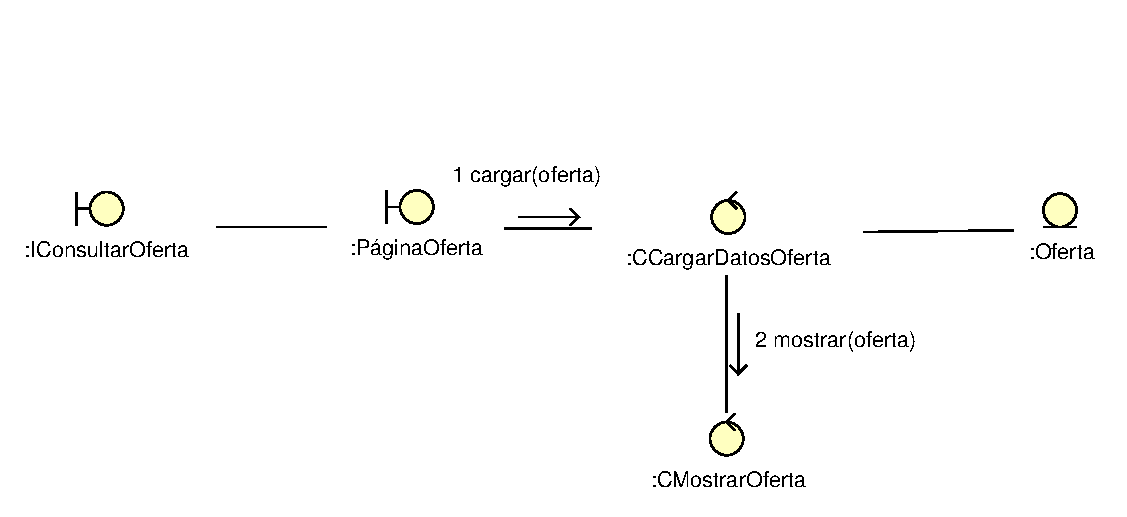
\includegraphics[scale=.85]{diagramas/consultaroferta.pdf}
				\end{figure}

			\subsubsection{Consultar vuelos}
				\begin{figure}[H]\centering
					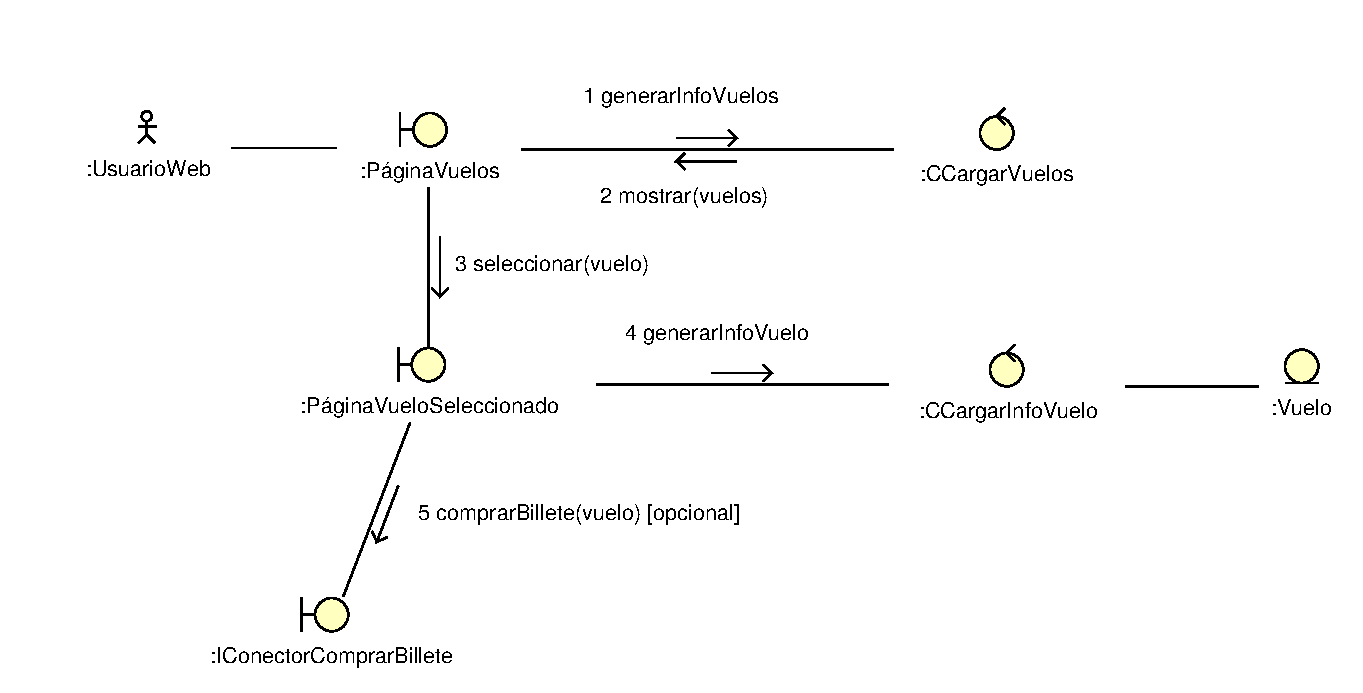
\includegraphics[scale=.71]{diagramas/consultarvuelos.pdf}
				\end{figure}
			
			\subsubsection{Editar datos personales}
				\begin{figure}[H]\centering
					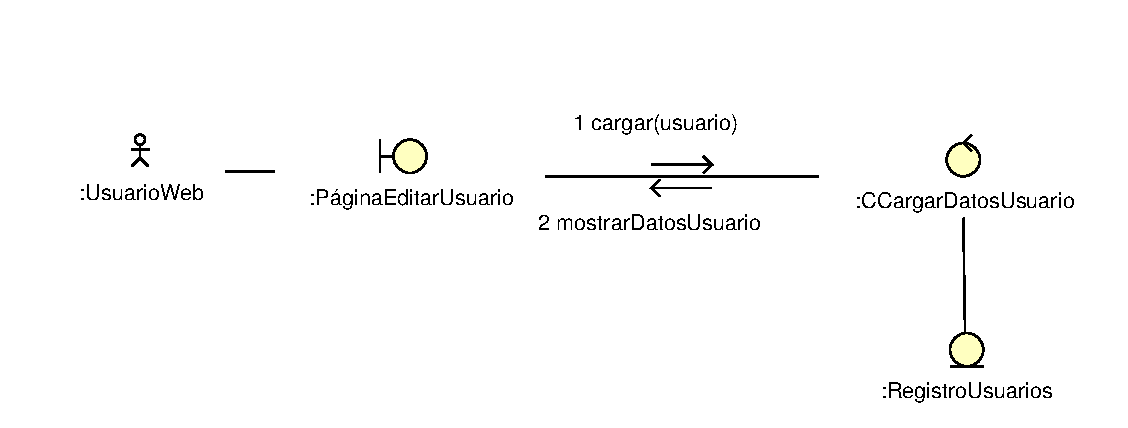
\includegraphics[scale=.86]{diagramas/editardatospersonales.pdf}
				\end{figure}


			\subsubsection{Iniciar pago billetes}
				\begin{figure}[H]\centering
					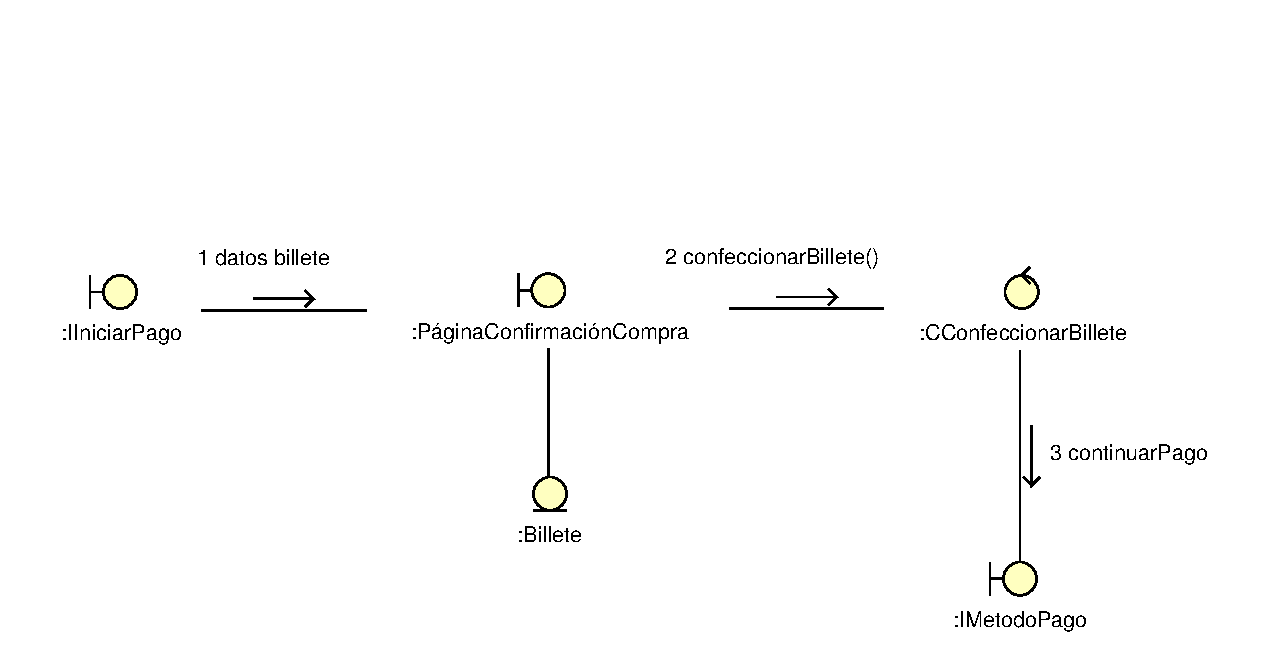
\includegraphics[scale=.76]{diagramas/iniciarpagobilletes.pdf}
				\end{figure}

					El caso de uso {\itshape Iniciar Pago de Billetes} recibe los datos de un billete de vuelo (en el diseño se ha generalizado a una asociación de billetes denominada {\itshape compra}) y tras mostrar una página de confirmación al usuario de las condiciones de la misma, se procede a la confección del billete y a la selección del método de pago\footnote{Realmente sólo se ha desarrollado un método de pago (\nameref{ana:tarjeta}) por lo que la selección del método se hace automáticamente.}. Finalmente el caso de uso se comunica con el método de pago seleccionado (a través de una interfaz conveniente) para continuar la operación.

			\subsubsection{Mostrar ofertas}
				\begin{figure}[H]\centering
					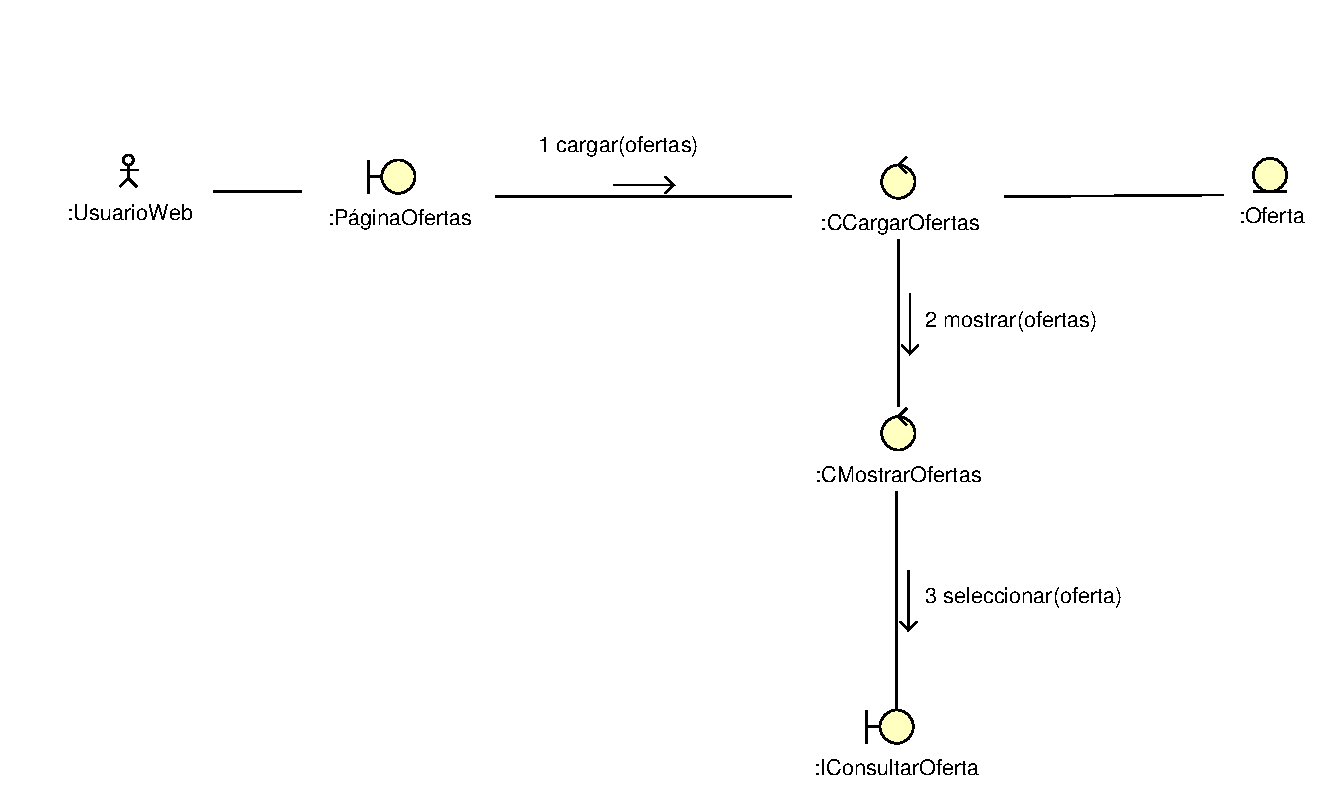
\includegraphics[scale=.72]{diagramas/mostrarofertas.pdf}
				\end{figure}

			\subsubsection{Realizar pago con tarjeta} \label{ana:tarjeta}
				\begin{figure}[H]\centering
					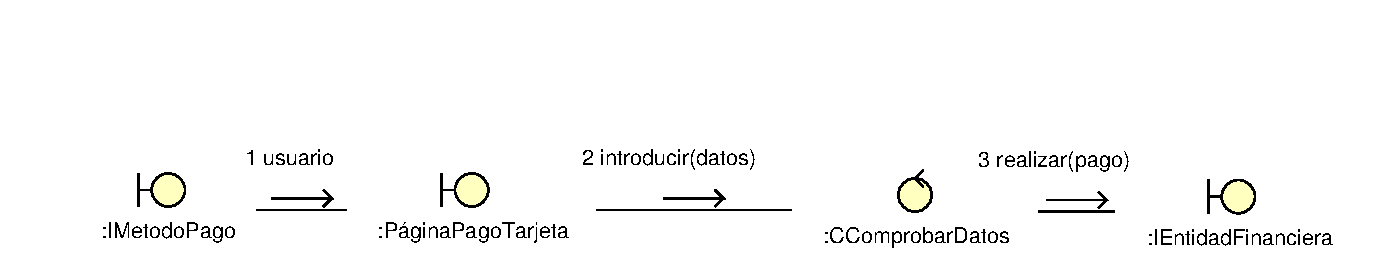
\includegraphics[scale=.7]{diagramas/pagotarjeta.pdf}
				\end{figure}

			\subsubsection{Presentar reclamación}
				\begin{figure}[H]\centering
					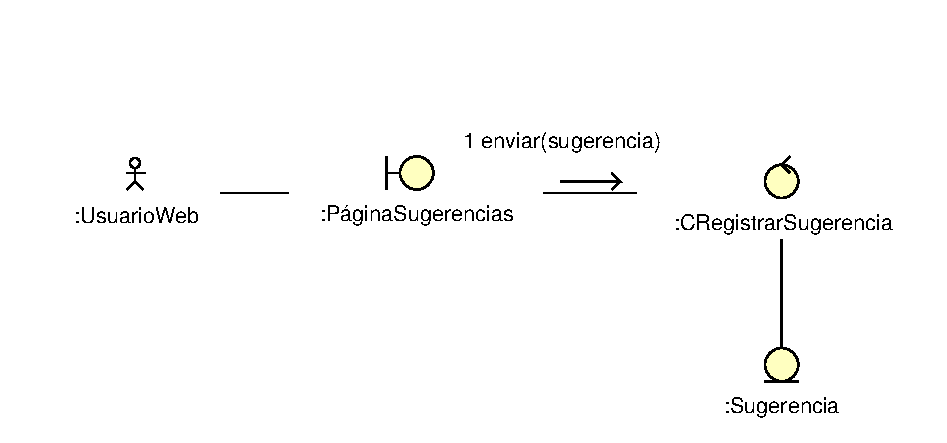
\includegraphics[scale=.82]{diagramas/presentarreclamacion.pdf}
				\end{figure}

			\subsubsection{Registrarse}
				\begin{figure}[H]\centering
					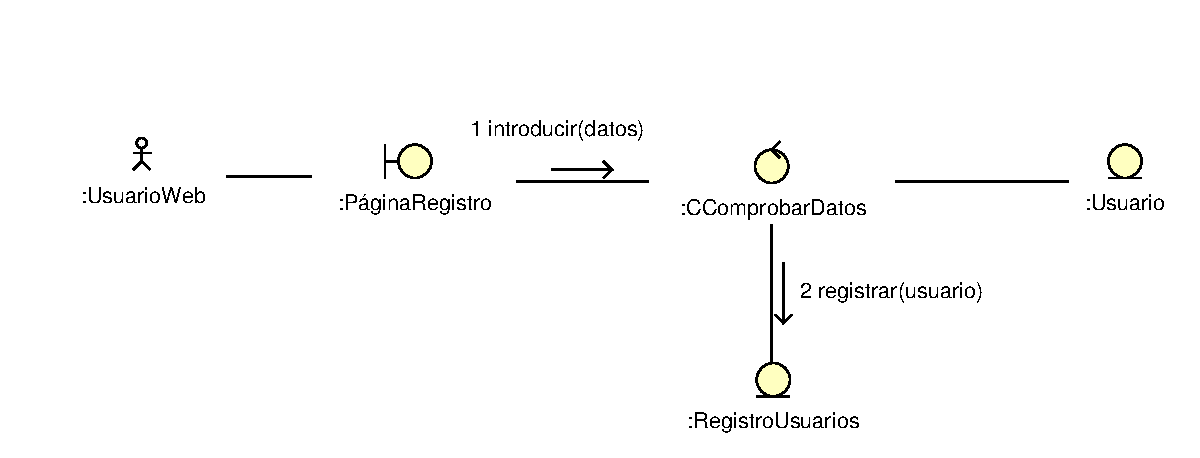
\includegraphics[scale=.8]{diagramas/registrarse.pdf}
				\end{figure}

			\subsubsection{Restablecer contraseña}
				\begin{figure}[H]\centering
					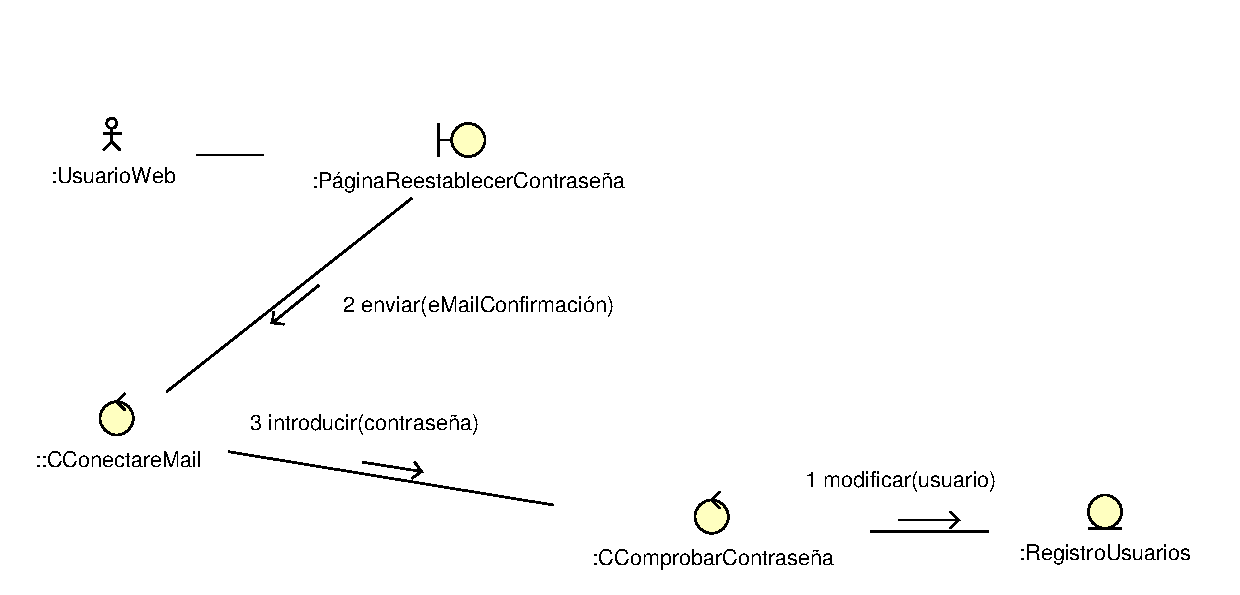
\includegraphics[scale=.77]{diagramas/restablecercontrasena.pdf}
				\end{figure}

			\subsubsection{Ver información de vuelo contratado}
				\begin{figure}[H]\centering
					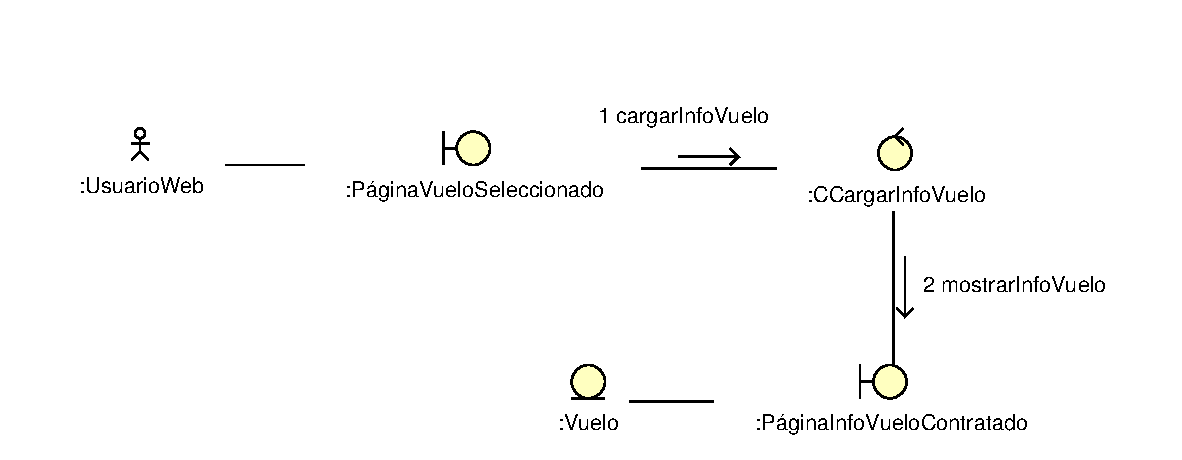
\includegraphics[scale=.8]{diagramas/verinfovuelocontratado.pdf}
				\end{figure}
\end{document}
